\section{Le logiciel de visualisation et d'analyse de l'internet}
\subsection{Objectifs}

Le but du projet est de produire un logiciel qui permette de visualiser tout ou partie de la topologie d'internet, ses points névralgiques % TODO orthographe
, , etc. 
Néanmoins, les objectifs du projet étaient plus pédagogiques.

\subsubsection{Objectif pédagogiques}
\paragraph{fixés : } L'objectif principal est bien évidemment d'apprendre à maîtriser la librairie boost de C++, en tout cas sa partie sur les graphs. Il était aussi question d'approfondir notre connaissance de la topologie d'internet.
\paragraph{improvisés : } De plus, nous nous sommes nous-même fixés des objectifs. En effet, l'utilisation d'une librairie graphique pour représenter la topologie d'internet était nécessaire mais son choix nous était réservé. Par conséquent nous avons choisi d'utiliser Qt, et ce pour deux raisons, la première c'est que nous voulions approfondir le cours sur Qt que nous allions avoir à l'ISIMA. 

La seconde est que, sous la pression de Nokia, cette librairie est récemment passé sous licence LGPL ce qui veut dire que les développeurs d'applications commerciales vont pouvoir développer gratuitement autour de Qt (sans payer les très onéreuses licences jusqu'à présent nécessaires pour vendre quelque chose en Qt). Il est fort probable que Qt prennent beaucoup plus d'ampleur dans les prochaines années.

\paragraph{} En outre, nous nous sommes fixés un autre objectif, celui d'apprendre à utiliser git, pour les raisons évoqué en \ref{gitPar} subversion ne nous convenait pas, mais nous ne connaissions pas vraiment git pour autant, néanmoins après avoir visionner une conférence de Linus Torvald sur le sujet, il nous a semblé logique et nécessaire d'appréhender git et de s'en servir pour le projet. D'autant plus que l'un comme l'autre nous avions effectué nos stages avec subversion ou cvs.

\subsubsection{La librairie graph de boost}

\subsubsection{La librairie graphique Qt}


\subsection{Méthodologie de développement et redistribution}
\subsubsection{Documentation avec Doxygen}
\subsubsection{Redistribution et travail en équipe}
\paragraph{subversion : des limites}
%TODO supprimer premier paragraphe
%EvOr se défoule
%La plupart des personnes ayant utilisé subversion de manière professionnelle en sont conscientes il est loin d'être agréable à utiliser, sa gestion des branches est désastreuses, et les conflits sont gérés de manière abruptes et souvent inefficaces, pour palier à ses défauts les entreprises mettent en place des politiques de fonctionnement autour du gestionnaire de version drastique avec par exemple interdiction de commiter ce qui ne marche pas. Au delà de ses problèmes de fonctionnement subversion est lent, très lent et nécessite en plus la présence d'un serveur pour pouvoir commiter.
%Fin EvOr se défoule

\paragraph{} L'une des bases du développement est d'utiliser un gestionnaire de sources afin de pouvoir modifier ses fichiers sans se soucier des conséquences. La première chose que nous avons faite, avant même de passer au développement, est de mettre en place un serveur subversion sur l'une de nos machines. Le problème qui s'est très vite posé est le suivant : quelque soit l'endroit où l'autre travaille, s'il n'a pas accès au serveur, il ne peut pas l'utiliser (\verb|commit/checkout|) et doit donc développer sans gestionnaire de sources (figure \ref{svn})... Il nous fallait un moyen de contrôler nos sources de manière distribuée : git.

\begin{figure}[H]
\begin{center}
        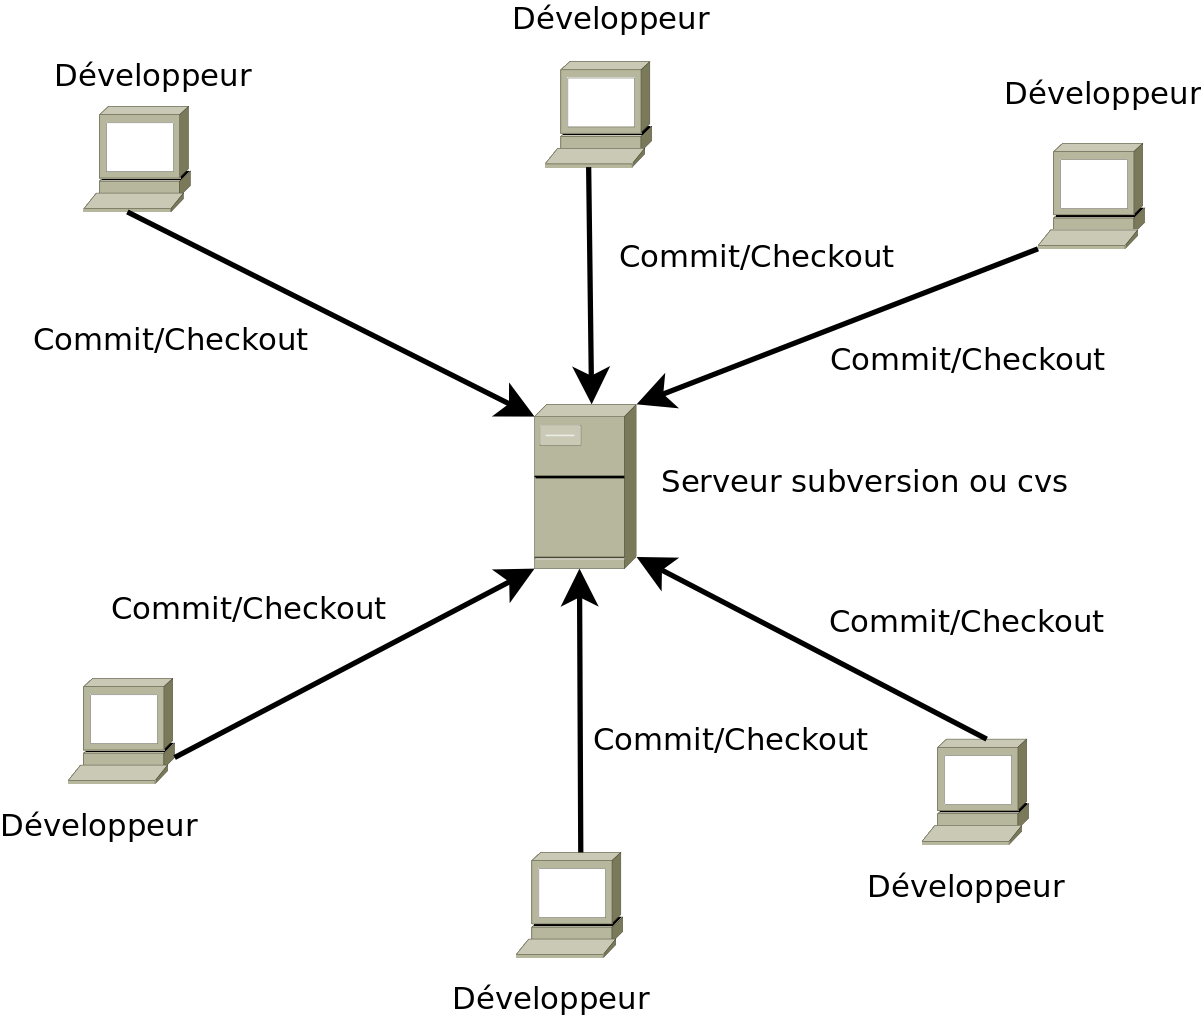
\includegraphics[width=0.7\textwidth]{../images/svn.png}
\caption{La gestion classique des sources : centralisation totale }
\label{svn}
\end{center}
\end{figure}


\paragraph{git : Le gestionnaire de source distribué}
\label{gitPar}
\paragraph{Histoire :}
\paragraph{} Git a été créé par Linus Torwald en 2004, il avait besoin de remplacer BitTracker pour la gestion des sources du noyau Linux, et il est évident qu'il ne peut pas mettre en place un serveur subversion pour un projet aussi vaste et avec autant de développeurs... Il a donc écrit en quelques jours un gestionnaire de sources distribué performant et qui a pour objectif de ne pas géner le développeur. En outre, Git effectue un checksum SHA1 des sources à chaque fois qu'une modifications est effectuée (commit ou push) ce qui permet d'être sûr de l'unicité des données...

\paragraph{Que veut dire distribué ?} 
\paragraph{}Git est distribué, cela veut dire que chaque machine l'utilisant est un serveur et un client. En d'autres termes chaque développeur peut commiter et effectuer des \verb|revert| en local. Ce qui permet de développer de manière beaucoup plus efficace, puisque les commits sont effectués en quelques millisecondes (le temps d'afficher la trace). Une fois que le développeur est satisfait de son travail, il peut demander aux autres de \verb|pull| (récupérer les sources) depuis sa machine, ou il peut \verb|push| (envoyer les sources) sur un serveur de fichiers centrales par exemple (figure \ref{git}). Tout ce que nécessite git pour fonctionner est un client et/ou un serveur ssh.


\begin{figure}[H]
\begin{center}
        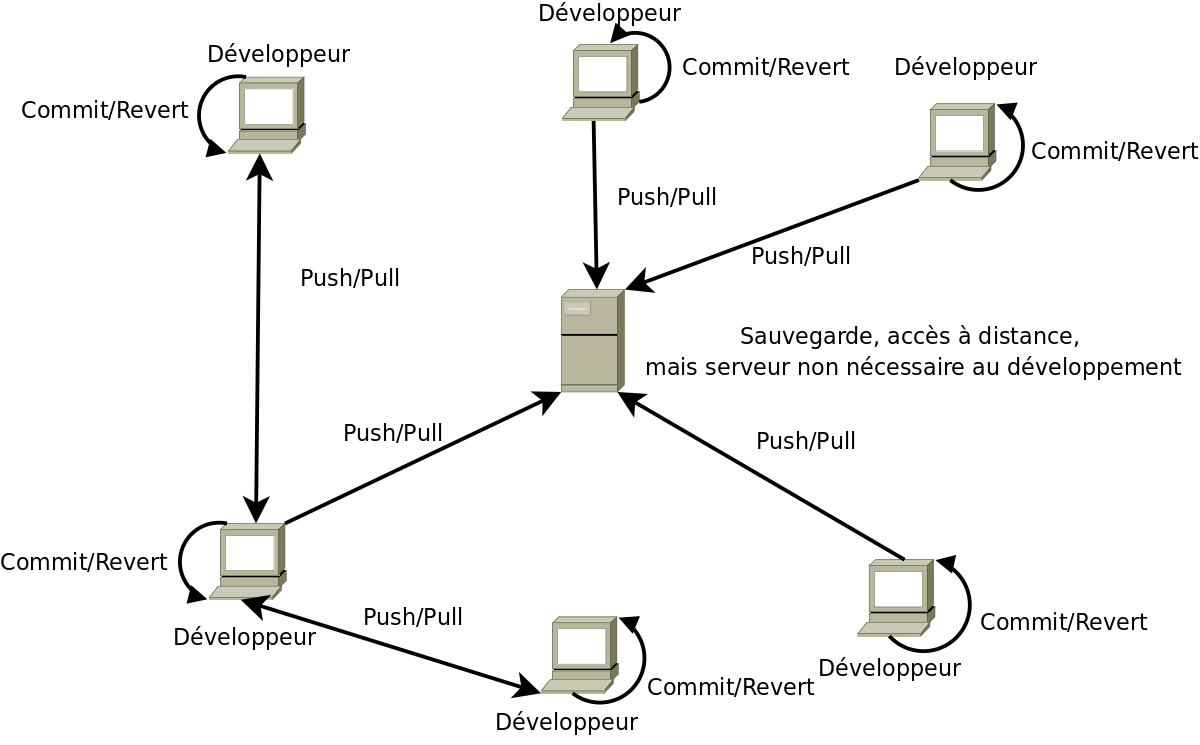
\includegraphics[width=0.8\textwidth]{../images/git.png}
\caption{La gestion des sources avec git : Distribution et liberté}
\label{git}
\end{center}
\end{figure}




\paragraph{Comment ça marche ?} 
\paragraph{}Concrètement, la clé du fonctionnement de git est l'utilisation massive des branches. En effet, dans git tout est une branche : chaque machine de chaque développeur est une branche et ce de manière totalement transparente. C'est à dire que le développeur peut \verb|commit| et \verb|revert| sa propre branche et l'envoyer ensuite sur la branche principale (\verb|master|) comme si c'était un simple commit de subversion. Avec les sources, l'historique des commits effectués en local est envoyé et n'importe quel développeur peut annuler n'importe quel commit. 

Il est donc très facile de créer, de merger et de supprimer une branche avec git, tellement facile qu'on se demande comment ça peut être aussi difficile avec subversion.

En cas de conflit, git ne fait rien ; pour git le simple fait que deux fichiers devant être ``mergés'' sont plus récents que leur dernière version commune est un conflit. Il signale alors à l'utilisateur qu'il faut ``merger''. Et ce merge est très aisé, il se déroule automatiquement souvent, à la main parfois : git est capable de ne montrer uniquement les parties de fichiers en conflit.

Nous vous renvoyons à nôtre annexe sur git pour un descriptif détaillé des commandes à connaître avec git.

%TODO en annexe les commandes de git
%Git fonctionne en ligne de commande, néanmoins ses développeur l'ont doté d'une interface graphique plutôt fonctionnelle. Git possède un nombre impressionant de fonctionnalités, nous allons toutefois lister celles qui nous semblemt les plus importantes.

\paragraph{Et l'accès aux données depuis l'extérieur ?}
\paragraph{} A l'instar de sourceforge pour subversion, il existe quelques sites communautaires permettant de déposer les sources de ses projets sur des serveurs distants, github en fait partie. En choisissant git, nous voulions, outre la puissance et la distribution, avoir accès aux modifications de l'un et de l'autre sans avoir besoin de s'appeler pour se demander d'allumer nos machines.

Centraliser nos sources sur la toile, nous a semblé être la meilleure solution. Github fonctionne avec git, il lui suffit d'avoir votre clé publique rsa et il est possible d'utiliser git avec le site. 

\paragraph{En résumé}

\paragraph{}L'utilisation conjuguée de git et de github nous permet donc :
\begin{itemize}
 \item De développer avec un gestionnaire de source sans accès au réseau ;
 \item D'avoir accès à notre projet par une simple commande quelque soit la machine sur laquelle nous travaillons ;
\item De développer avec un outil puissant, rapide et efficace.
\end{itemize}

\subsection{Aperçu du logiciel}
\subsubsection{Modèle Vue Controlleur}
Lorsque l'on développe une application disposant d'une interface graphique, la base du développement est de séparer la partie traitement ou métier de l'interface à proprement parler. Il est souvent utile de rajouter une couche d'interfaçage entre la partie métier et la partie affichage. Cette modélisation s'appelle Modèle Vue Controlleur. Nous avons choisi d'implémenter ce modèle dans notre projet. La partie métier étant le graph représentant les AS de l'internet et leur liens. Un schéma très superficiel du pattern est présenté en figure \ref{mvc}.

L'utilisation que nous avons faites de l'objet Graph une fois créé, analysé et rempli, peut être assimiler à l'accès à une base de données. L'ensemble des méthodes d'accès se trouvant dans le controler, la partie métier n'en a absolument aucune connaissance. De même, la partie affichage n'a accès qu'aux méthodes du controlleur.

Le but de ce pattern est de permettre aux développeurs de changer la vue en ne modifiant aucune autre partie du code, ou de modifier la partie métier sans modifier le code de la vue. En outre, un tel découpage facilite la répartition des tâches dans l'équipe.

\begin{figure}[H]
\begin{center}
        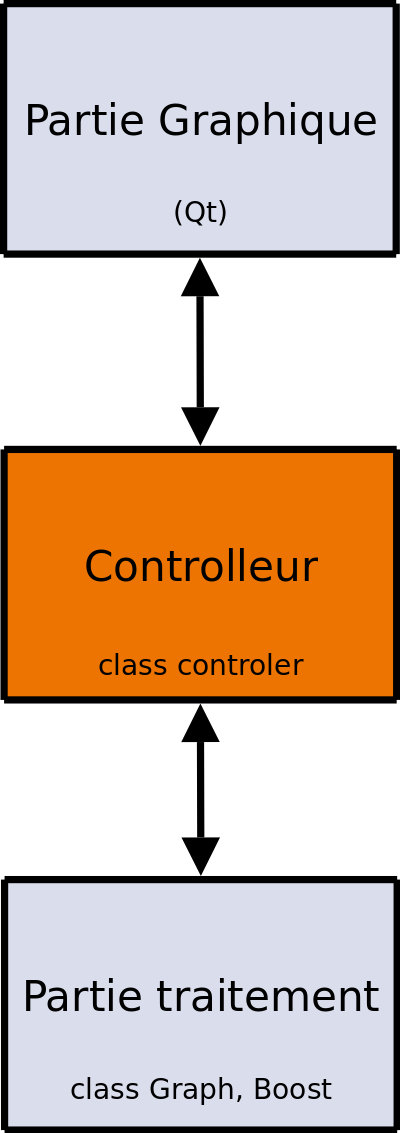
\includegraphics[height=0.3\textheight]{../images/mvcScheme.png}
\caption{Schéma superficiel du Modèle Vue Controlleur}
\label{mvc}
\end{center}
\end{figure}
\subsubsection{Répartition des tâches}




\subsubsection{Première idée de représentation}


